% Template KLTN cho SV trường ĐHKHTN
% Liên hệ: nqminh@fit.hcmus.edu.vn
% Last update: 30/11/2016

% Chú ý: đọc các phần chú ý đóng khung của file này và chỉnh lại cho phù hợp.
% Trước khi build, xóa hết các file được tạo ra trong quá trình build trước đó (tất cả các file nằm ở thư mục gốc, trừ file main.tex này), và build theo thứ tự: BIB > PDF > PDF.
% Nếu cập nhật tài liệu tham khảo, cũng cần build lại theo cách trên.

% Đã kiểm tra trên MikTeX 2.9 Windows, TexMaker, Winshell

\documentclass[oneside,a4paper,12pt]{extreport}

% Font tiếng Việt
\usepackage[T5]{fontenc}
\usepackage[utf8]{inputenc}
\DeclareTextSymbolDefault{\DH}{T1}

% Tài liệu tham khảo
\usepackage[
	sorting=nty,
	backend=bibtex,
	defernumbers=true]{biblatex}
\usepackage[unicode]{hyperref} % Bookmark tiếng Việt
\addbibresource{References/references.bib}

\makeatletter
\def\blx@maxline{77}
\makeatother

% Chèn hình, các hình trong luận văn được để trong thư mục Images/
\usepackage{graphicx}
\graphicspath{ {Images/} }

% Chèn và định dạng mã nguồn
\usepackage{listings}
\usepackage{color}
\definecolor{codegreen}{rgb}{0,0.6,0}
\definecolor{codegray}{rgb}{0.5,0.5,0.5}
\definecolor{codepurple}{rgb}{0.58,0,0.82}
\definecolor{backcolour}{rgb}{0.95,0.95,0.92}
\lstdefinestyle{mystyle}{
    backgroundcolor=\color{backcolour},   
    commentstyle=\color{codegreen},
    keywordstyle=\color{magenta},
    numberstyle=\tiny\color{codegray},
    stringstyle=\color{codepurple},
    basicstyle=\footnotesize,
    breakatwhitespace=false,         
    breaklines=true,                 
    captionpos=b,                    
    keepspaces=true,                 
    numbers=left,                    
    numbersep=5pt,                  
    showspaces=false,                
    showstringspaces=false,
    showtabs=false,                  
    tabsize=2
}
\lstset{style=mystyle}

% Chèn và định dạng mã giả
\usepackage{amsmath}
\usepackage{algorithm}
\usepackage[noend]{algpseudocode}
\makeatletter
\def\BState{\State\hskip-\ALG@thistlm}
\makeatother

% Bảng biểu
\usepackage{multirow}
\usepackage{array}
\usepackage{booktabs}
\newcolumntype{L}[1]{>{\raggedright\let\newline\\\arraybackslash\hspace{0pt}}m{#1}}
\newcolumntype{C}[1]{>{\centering\let\newline\\\arraybackslash\hspace{0pt}}m{#1}}
\newcolumntype{R}[1]{>{\raggedleft\let\newline\\\arraybackslash\hspace{0pt}}m{#1}}

% Đổi tên mặc định
%\renewcommand{\chaptername}{Chương}
%\renewcommand{\figurename}{Hình}
%\renewcommand{\tablename}{Bảng}
%\renewcommand{\contentsname}{Mục lục}
%\renewcommand{\listfigurename}{Danh sách hình}
%\renewcommand{\listtablename}{Danh sách bảng}
%\renewcommand{\appendixname}{Phụ lục}

% Dãn dòng 1.5
\usepackage{setspace}
\onehalfspacing

% Thụt vào đầu dòng
\usepackage{indentfirst}

% Canh lề
\usepackage[
  top=35mm,
  bottom=30mm,
  left=35mm,
  right=20mm,
  includefoot]{geometry}
  
% Trang bìa
\usepackage{tikz}
\usetikzlibrary{calc}
\newcommand\HRule{\rule{\textwidth}{1pt}}

% ========================================================================================= %
% CHÚ Ý: Thông tin chung về KLTN - sinh viên điền vào đây để tự động update các trang khác  %
% ========================================================================================= %
\newcommand{\tenSV}{Thai~Thien} % Dấu ~ là khoảng trắng không được tách (các chữ nối với nhau bằng dấu ~ sẽ nằm cùng 1 dòng
\newcommand{\mssv}{1351040}
\newcommand{\tenSVt}{Van~Duy~Vinh} % Dấu ~ là khoảng trắng không được tách (các chữ nối với nhau bằng dấu ~ sẽ nằm cùng 1 dòng
\newcommand{\mssvt}{1351050}
\newcommand{\tenKL}{Sử~dụng~LaTeX trong Khoá~luận~tốt~nghiệp} % Chú ý dấu ~ trong tên khóa luận
\newcommand{\tenGVHD}{Nghiêm Quốc Minh}
\newcommand{\tenBM}{Công nghệ tri thức}

\begin{document}

\begin{titlepage}

\begin{center}
UNIVERSITY OF SCIENCE\\
ADVANCED PROGRAM IN COMPUTER SCIENCE\\[2cm]
%BỘ MÔN \MakeUppercase{\tenBM}\\[2cm]

{ \Large \bfseries \MakeUppercase{\tenSV ~-~ \mssv} \\[2cm]
\Large \bfseries \MakeUppercase{\tenSVt ~-~ \mssvt} } %Nếu có 2 sinh viên thì chèn thêm 1 dòng vào đây, đồng thời chú ý canh trang cho phù hợp

{ \LARGE \bfseries \MakeUppercase{\tenKL} \\[2cm] } %SV có thể tự điền tên vào nếu cần xuống dòng chỗ phù hợp

\Large BACHELOR OF SCIENCE IN COMPUTER SCIENCE\\[2cm]

%\Large GIÁO VIÊN HƯỚNG DẪN\\
%\MakeUppercase{\tenGVHD} \\[2cm]

\begin{tikzpicture}[remember picture, overlay]
  \draw[line width = 2pt] ($(current page.north west) + (2cm,-2cm)$) rectangle ($(current page.south east) + (-1.5cm,2cm)$);
\end{tikzpicture}

\vfill
HO CHI MINH CITY, \the\year

\end{center}

\end{titlepage}


\begin{titlepage}

\begin{center}
UNIVERSITY OF SCIENCE\\
ADVANCED PROGRAM IN COMPUTER SCIENCE\\[2cm]
%BỘ MÔN \MakeUppercase{\tenBM}\\[2cm]

{ \Large \bfseries \MakeUppercase{\tenSV ~-~ \mssv} \\
\Large \bfseries \MakeUppercase{\tenSVt ~-~ \mssvt} \\[2cm] } %Nếu có 2 sinh viên thì chèn thêm 1 dòng vào đây, đồng thời chú ý canh trang cho phù hợp
 
{ \LARGE \bfseries \MakeUppercase{\tenKL} \\[2cm] } %SV có thể tự điền tên vào nếu cần xuống dòng chỗ phù hợp

\Large BACHELOR OF SCIENCE IN COMPUTER SCIENCE\\[2cm]

\Large THESIS ADVISOR\\
\MakeUppercase{\tenGVHD} \\[2cm]

\begin{tikzpicture}[remember picture, overlay]
  \draw[line width = 2pt] ($(current page.north west) + (2cm,-2cm)$) rectangle ($(current page.south east) + (-1.5cm,2cm)$);
\end{tikzpicture}

\vfill
HO CHI MINH CITY, \the\year

\end{center}

\end{titlepage}

% Sasu trang Title, các bạn chèn nhận xét gủa GVHD và GVPB. Nhận xét sẽ được giáo vụ phát sau buổi bảo vệ để các bạn đóng quyển.

\pagenumbering{roman} % Đánh số i, ii, iii, ...

%\addcontentsline{toc}{chapter}{Lời cam đoan}
%\chapter*{Lời cam đoan}
\label{reassurances}

Tôi xin cam đoan đây là công trình nghiên cứu của riêng tôi. Các số liệu và kết quả nghiên cứu trong luận văn này là trung thực và không trùng lặp với các đề tài khác.

\addcontentsline{toc}{chapter}{ACKNOWLEDGMENTS}
\chapter*{ACKNOWLEDGMENTS}
\label{thanks}

Tôi xin chân thành cảm ơn~\ldots

Xin cám ơn!

\vspace{3cm}
\hspace{7cm}
\begin{minipage}[ht]{0.48\textwidth}
\begin{center}
Tp. Hồ Chí Minh, ngày ... tháng ... năm 2016

Sinh viên thực hiện

\tenSV  ~~~~~~~   \tenSVt 
\end{center}
\end{minipage}


%\addcontentsline{toc}{chapter}{Đề cương chi tiết}
%\begin{flushleft}
Khoa Công Nghệ Thông Tin\\
Bộ môn \tenBM\\[2cm]
\end{flushleft}

\begin{center}
\LARGE \textbf{ĐỀ CƯƠNG CHI TIẾT}
\end{center}

\begin{tabular}{|L{15cm}|}
\hline
\textbf{Tên đề tài:} \tenKL \\
\hline
\textbf{Giáo viên hướng dẫn:} \tenGVHD \\
\hline
\textbf{Thời gian thực hiện:} 01/01/2000-01/01/2001\\
\hline
\textbf{Sinh viên thực hiện:}
 \tenSV ~-~ \mssv \\
 \tenSVt ~-~ \mssvt \\
\hline
\textbf{Loại đề tài:} Tìm hiểu công nghệ (có hoặc không ứng dụng minh hoạ), Xây dựng ứng dụng, ...\\
\hline
\end{tabular}\\[1cm]

\begin{tabular}{|L{15cm}|}
\hline
\textbf{Nội dung đề tài:} mô tả chi tiết nội dung đề tài, yêu cầu, phương pháp thực hiện, kết quả đạt được, ...\\
\hline
\textbf{Kế hoạch thực hiện:} mô tả chi tiết thời gian của các giai đoạn thực hiện và phân công công việc của từng thành viên trong nhóm\\
\hline
\end{tabular}\\[1cm]

\begin{tabular}{C{8cm}C{8cm}}
Xác nhận của GVHD & Ngày ... tháng ... năm 2016 \\
    ~\\~          & ~\\~                        \\
\tenGVHD          & \tenSV  ~~~~~~~~~~~~~~~~ \tenSVt
\end{tabular}


% Mục lục, danh sách hình, danh sách bảng
\addcontentsline{toc}{chapter}{TABLE OF CONTENTS}
\tableofcontents
\listoffigures
\listoftables

\addcontentsline{toc}{chapter}{ABSTRACT}
\chapter*{ABSTRACT}
\label{tomtat}

A large proportion of our perceptions of the world around us is made up of opinions.
In large scale, opinions run our economy, shape our government and drive our history.
The ability to comprehend and control opinions brings great power.
Since the last decade, opinions have been expressed in the highest speed, volume, and complexity ever recorded in history.
As a result, the task of tracking the flow of opinions on the Internet become impossible without automation.
To fill the niche, Sentiment Analysis is the field of study that investigates the computational method for analyzing opinions.
In this field, one significant problem is to classify the sentiment expressed by a sentence.
This problem is named Sentence-level Sentiment Analysis.

The purpose of this thesis is to increase the classification accuracy on the task of sentence-level Sentiment Analysis.
For this purpose, three approaches were explored.
In the first approach, we tried to improve Recursive Neural Networks by parameterizing their composition functions with respect to local syntactic information at each node in the parse tree.
For our second approach, we recognized that one major obstacle of this task is the lack of context and knowledge in the small training set.
To tackle this problem, we utilized Glove method to do Transfer Learning on a large amount of document-level labeled sentiment data.
In the third approach, we combined Convolution Neural Networks with Recursive Neural Networks, which result in new sophisticated networks architect.
To mitigate the risk posed by training large networks on small training dataset, we experimented with several unsupervised pre-training methods which also types of Transfer Learning.

We evaluated our models on the public Stanford Sentiment Treebank dataset with binary setting.
We were able to outperform the state-of-the-art model by a good margin in terms average accuracy of 5 runs.


\clearpage

\pagenumbering{arabic} % Đánh số 1, 2, 3, ...

% Các chương nội dung
\chapter{Introduction}


\chapter{Technical Issues}
\section{Framework}

\subsection{Torch}
Torch \footnote{http://torch.ch/} is Lua scientific computing framework. Torch support high performing matrix calculation via multi-dimensional array call Tensor. Torch are built with C/C++, CUDA backend. Torch author choose Lua because Lua works well with C/C++ \cite{collobert2011torch7}.  Thus, Torch is high performing and support GPU. Torch have neural network package (nn) package. Computation graph must be define before forward pass. 
A simple, single linear layer network can be easily defined with few line of code (see listing \ref{lst:torchlinear}).

\begin{lstlisting}[caption={Simple linear layer in Torch},label={lst:torchlinear}, language={[5.1]Lua}]
-- simple y = Ax + b linear layer
l = nn.Linear(2,3)
-- forward pass
x = torch.Tensor(2)
y = l:forward(x) -- vector dimension of 3
\end{lstlisting}

However, when a model need multiple module, such as multilayer perceptron (MLP), these module must be put into container. Figure \ref{fig:nncontainer} illustrates on function of each nn container . In order to construct two-layer perception (eq \ref{eq:mlp}), linear, tanh and softmax module must be packed into sequential module (see listing \ref{lst:torchmlp}).

\begin{equation}
\label{eq:mlp}
\begin{aligned}
&h = tanh(W_1*x + b_1) \\
&y = softmax(W_2*h + b2)
\end{aligned}
\end{equation}


\begin{lstlisting}[caption={MLP in Torch},label={lst:torchmlp}, language={[5.1]Lua}]
model = nn.Sequential()
model:add(nn.Linear(2,3))
model:add(nn.Tanh())
model:add(nn.Linear(3,5))
model:add(nn.SoftMax())
-- forward
x = torch.Tensor(2)
y = model:forward(x)
\end{lstlisting}

Torch provide nngraph package support build more complicate model. For example, define MLP in (eq \ref{eq:mlp}) use nngraph (see listing \ref{lst:torchnngraph})

\begin{lstlisting}[caption={MLP using nngraph},label={lst:torchnngraph}, language={[5.1]Lua}]
model = nn.Sequential()
model:add(nn.Linear(2,3))
model:add(nn.Tanh())
model:add(nn.Linear(3,5))
model:add(nn.SoftMax())
-- forward
x = torch.Tensor(2)
y = model:forward(x)
\end{lstlisting}

Sample code on training a model, see Appendix \ref{lst:torchtrain}

\subsection{Theano}
Theano \footnote{\url{http://deeplearning.net/software/theano/}} is a deep learning library on Python. It basic function is similar to Torch: matrix calculation, support GPU. Theano is define-and-run schema, which a computer graph must be built before it is executed.

\begin{lstlisting}[caption={Define function in Theano},label={lst:theanof}, language={python}]
x = T.dmatrix('x')
y = T.dmatrix('y')
z = x + y
f = function([x, y], z)
f([[1, 1], [2, 2]], [[3, 3], [4, 4]])
# result [[4, 4], [6, 6]]
\end{lstlisting}

Comparing to Torch7, Theano are slower on most benchmark \cite{collobert2011torch7}. Theano does not provide nice template like linear layer. Thus, model must be defined from equation. It give researcher more control over mathematics aspect but cause more trouble for beginner. A sample code for MLP \ref{lst:theanomlp}. One more problem is that the 'define-and-run' scheme does not suitable for recursive neural network due to recompile the computation graph each training sample take time. 

\subsection{Pytorch}
PyTorch uses same backend as Torch. However, PyTorch specially designed for Python. Pytorch have pre-define module (Linear layer, Convolution layer) like Torch. However, Pytorch does not require to pack model into container. In Pytorch a network are defined in forward-pass thanks to Dynamic Neural Networks feature. Therefore, user can use Python control flow to define a network. For example, one can use for loop to run recurrent neural network (see ) .The features allows us to implement Recursive Neural Network for NLP, which the network change for every sample, much more easier. 

\begin{lstlisting}[caption={RNN},label={lst:pytorchrnn}, language={python}]
rnn = torch.
\end{lstlisting}




\chapter{Experiment}

\section{Dataset}

\subsection{Stanford Sentiment Treebank}
In this thesis, we use Standford Sentiment Treebank (SST) dataset \cite{socher2013recursive}. Standford Sentiment Treebank contains 11,855 sentences. Each data sentence consist of fined-grain sentiment labeled phrases in constituency parse tree structure (see \textbf{Figure \ref{fig:sst}}). There are total 215,154 phrases in whole dataset.
The dataset was splitted into train/dev/test contain 8544/1101/2210 sentences each for training and evaluation models. After remove neutral sentiment sentences, there are 6920/872/1821 sentences remained in train/dev/test set.

SST dataset are publicly available online \footnote{https://nlp.stanford.edu/sentiment/index.html}.

\subsubsection{Preprocess}
We use preprocess source code from \cite{socher2013recursive} implementation \footnote{\url{https://github.com/stanfordnlp/treelstm}} to preprocess SST.



\subsection{Amazon Movies Review}
We get Amazon Movies and TV reviews (4,607,047 reviews) and Amazon Book reviews (22,507,155 reviews) \cite{he2016ups}. Listing \ref{lst:amzrevie} is sample of one book review.

%TODO: change to book example
\begin{lstlisting}[caption={Amazon reviews sample},label={lst:amzreview}]
	{
	  "reviewerID": "A2SUAM1J3GNN3B",
	  "asin": "0000013714",
	  "reviewerName": "J. McDonald",
	  "helpful": [2, 3],
	  "reviewText": "I bought this for my husband who plays the piano.  He is having a wonderful time playing these old hymns.  The music  is at times hard to read because we think the book was published for singing from more than playing from.  Great purchase though!",
	  "overall": 5.0,
	  "summary": "Heavenly Highway Hymns",
	  "unixReviewTime": 1252800000,
	  "reviewTime": "09 13, 2009"
	}
\end{lstlisting}

We extract reviewText and overall from review dataset. We use overall as sentiment score for reviews, with 5 is very positive and 0 is very negative.



% how to preprocess amazon movies reviews
We get Amazon Movies and TV reviews (4,607,047 reviews) and Amazon Book reviews (22,507,155 reviews) \cite{he2016ups} as our training dataset for our word embedding layer. First, we join both dataset and shuffle. Then, we group review of same produce together. Finally, for each product, we sort reviews based on score. Hence, neighbor reviews have similar sentiment and talk about same product, except at the boundary of two produces. We also create one version of dataset which we only shuffle the data without group or sort for comparision. We train our word representation from Amazon dataset using Glove \cite{pennington2014glove} on 15 iteration with windows size of 20.


\begin{figure}[H]
	\begin{minipage}{\textwidth}
		\centering
		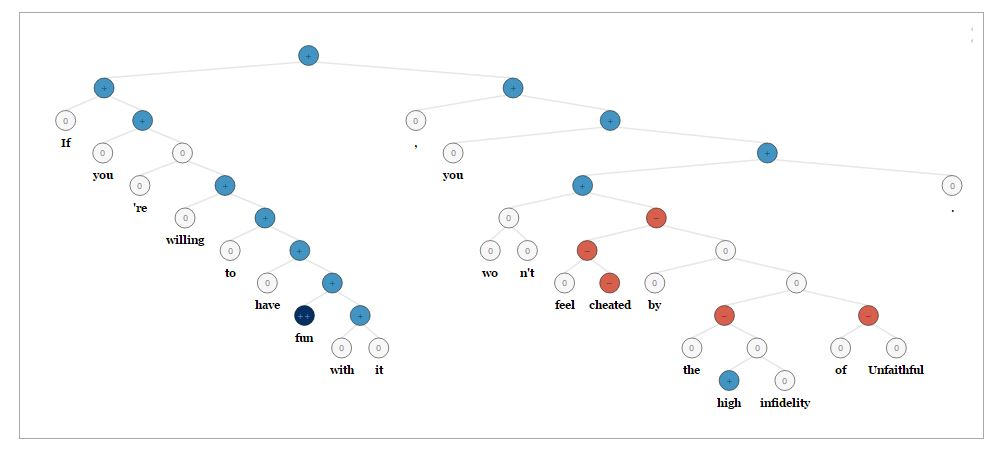
\includegraphics[width=0.9\linewidth]{figure/sst}
		\caption[A parsed sentence in SST]{A parsed sentence in SST \footnote{Render by Pytreebank \url{https://github.com/JonathanRaiman/pytreebank}}}
		\label{fig:sst}
	\end{minipage}
\end{figure}



\section{Embedding}
We run experiment on variety of pre-trained word representation.

\section{title}

% Please add the following required packages to your document preamble:
% \usepackage{booktabs}
% Please add the following required packages to your document preamble:
% \usepackage{booktabs}
\begin{table}[]
	\centering
	\caption{My caption}
	\label{my-label}
	\begin{tabular}{@{}lll@{}}
		\toprule
		& Constituency Tree-LSTM & LSTM \\ \midrule
		Glove 42B             &                        &      \\
		Glove 840B            &                        &      \\
		Glove (Amazon)        &  88.45           &      \\
		Glove (Amazon Sorted) &  88.85           &      \\
		Paragram-Phrase XXL   &                        &      \\
		SSWEu                 &                        &      \\ \bottomrule
	\end{tabular}
\end{table}


% Công trình của tác giả (nếu không có thì comment 02 dòng dưới)
\addcontentsline{toc}{chapter}{Danh mục công trình của tác giả}
\chapter*{Danh mục công trình của tác giả}
\label{Appendix1}

\begin{enumerate}
\item Tạp chí ABC
\item Tạp chí XYZ
\end{enumerate}

% In tài liệu tham khảo
\addcontentsline{toc}{chapter}{TABLE OF CONTENTS}
\printbibheading[title={TABLE OF CONTENTS}]

\printbibliography[heading=subbibliography, title={Vietnamese}, keyword=Viet, resetnumbers=true]

\DeclareNameAlias{sortname}{last-first}
\DeclareNameAlias{default}{last-first}

\printbibliography[heading=subbibliography, title={English}, notkeyword=Viet, resetnumbers=4] 
% ===================================================================== %
% CHÚ Ý: phải gán lại resetnumbers=số tài liệu tham khảo tiếng Việt + 1 %
% ===================================================================== %

% Phần phụ lục
\appendix

\chapter{APPENDICES 1}
\label{Appendix1}

\begin{figure} [H]
	\begin{minipage}{\textwidth}
		\centering
		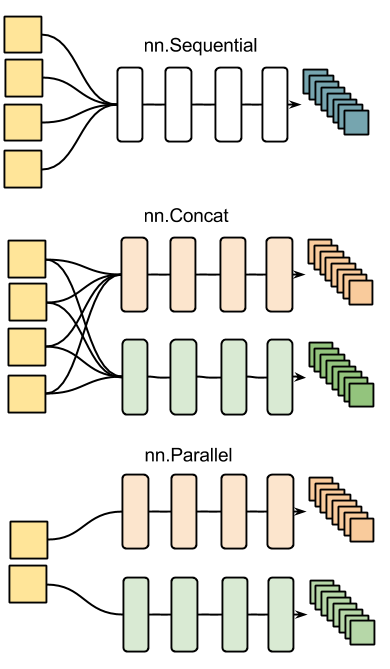
\includegraphics[width=0.5\linewidth]{figure/nncontainer}
		\caption[Torch nn container]{Torch nn container \footnote{ \url{https://github.com/soumith/cvpr2015/blob/master/Deep\%20Learning\%20with\%20Torch.ipynb}}}
		\label{fig:nncontainer}
	\end{minipage}
\end{figure}

\begin{lstlisting}[caption={MLP using nngraph},label={lst:torchtrain}, language={[5.1]Lua}]
require 'nn'
require 'optim'

model = nn.Sequential()
model:add(nn.Linear(1,1))

criterion = nn.MSECriterion()

x = torch.Tensor{{1,2,3,4,5,6,7,8,9,10}}
x = x:t()
y = torch.Tensor{{3,5,7,9,11,13,15,17,19,21}}
y = y:t()

params, gradParams = model:getParameters()

function feval(params)
gradParams:zero()
local outputs = model:forward(x)
local loss = criterion:forward(outputs,y)
local dloss_doutput = criterion:backward(outputs,y)
model:backward(x, dloss_doutput)
return loss, gradParams
end

local optimState = {
learningRate = 0.01
}

for epoch = 1, 100 do
optim.sgd(feval,params, optimState)
end

test = torch.Tensor{{1,3,5,7,9,11,100}}
test = test:t()

print (model:forward(test))
\end{lstlisting}



\begin{lstlisting}[caption={Theano MLP},label={lst:theanomlp}, language={python}]
import numpy as np
import theano
import theano.tensor as T
import theano.tensor.nnet as nnet

class MLP:
def __init__(self):
x = T.dvector()
y = T.dscalar()
t1 = np.array(np.random.rand(3, 3), dtype=theano.config.floatX)
theta1 = theano.shared(t1)  # 3x3 weight matrix
t2 = np.array(np.random.rand(4, 1), dtype=theano.config.floatX)
hid1 = MLP.sigmoid_layer(x, theta1)  # hidden layer
theta2 = theano.shared(t2)  # 4x1 weight matrix
output_layer = T.sum(MLP.sigmoid_layer(hid1, theta2))
fc = (output_layer - y)**2
self.cost = theano.function(inputs=[x,y], outputs = fc,updates=[
(theta1, Xor.grad_desc(fc, theta1)),
(theta2, Xor.grad_desc(fc, theta2))
])
self.run_forward = theano.function(inputs=[x],outputs=output_layer)

@staticmethod
def sigmoid_layer(x, w):
b = np.array([1], dtype=theano.config.floatX)
new_x = T.concatenate([x,b])
m = T.dot(w.T, new_x)
h = nnet.sigmoid(m)
return h


@staticmethod
def grad_desc(cost, theta):
alpha = 0.1
return theta - (alpha* T.grad(cost, wrt=theta))

def forward(self, x):
output = self.run_forward(x)
return output


def train(self, train_x, train_y, n_epoch):
cur_cost = 0
for epoch in range(n_epoch):
for i in range(len(train_x)):
cur_cost = self.cost(train_x[i],train_y[i])
if epoch % 1000 == 0:
print(cur_cost)
print ('train complete')
\end{lstlisting}

\chapter{APPENDICES 2}
\label{Appendix2}

Đây là phụ lục 2.

\end{document} 